\documentclass[fontsize=12pt]{scrartcl}
\usepackage{../mypack}
\usepackage{animate}
\usepackage{courier}
\usepackage{listings}
\usepackage[toc,page,title,titletoc]{appendix}
\definecolor{mygreen}{rgb}{0,0.6,0}
\definecolor{mygray}{rgb}{0.5,0.5,0.5}

\definecolor{mymauve}{rgb}{0.58,0,0.82}
\lstset{ %
  backgroundcolor=\color{white},   % choose the background color; you must add \usepackage{color} or \usepackage{xcolor}; should come as last argument
  basicstyle=\footnotesize\ttfamily,        % the size of the fonts that are used for the code
  breakatwhitespace=false,         % sets if automatic breaks should only happen at whitespace
  breaklines=true,                 % sets automatic line breaking
  captionpos=b,                    % sets the caption-position to bottom
  commentstyle=\color{mygreen},    % comment style
  %deletekeywords={...},            % if you want to delete keywords from the given language
  %escapeinside={\%*}{*)},          % if you want to add LaTeX within your code
  extendedchars=true,              % lets you use non-ASCII characters; for 8-bits encodings only, does not work with UTF-8
  %frame=single,	                   % adds a frame around the code
  keepspaces=true,                 % keeps spaces in text, useful for keeping indentation of code (possibly needs columns=flexible)
  keywordstyle=\color{blue},       % keyword style
  language=python,                 % the language of the code
  %morekeywords={*,...},            % if you want to add more keywords to the set
  xleftmargin=.04\textwidth,  
  numbers=left,                    % where to put the line-numbers; possible values are (none, left, right)
  numbersep=5pt,                   % how far the line-numbers are from the code
  numberstyle=\tiny\color{mygray}, % the style that is used for the line-numbers
  rulecolor=\color{black},         % if not set, the frame-color may be changed on line-breaks within not-black text (e.g. comments (green here))
  showspaces=false,                % show spaces everywhere adding particular underscores; it overrides 'showstringspaces'
  showstringspaces=false,          % underline spaces within strings only
  showtabs=false,                  % show tabs within strings adding particular underscores
  stepnumber=1,                    % the step between two line-numbers. If it's 1, each line will be numbered
  stringstyle=\color{mymauve},     % string literal style
  tabsize=4,	                   % sets default tabsize to 2 spaces
  %title=\lstname                   % show the filename of files included with \lstinputlisting; also try caption instead of title
}


\Autoren{Andreas Wilhelm}
\VersuchLang{Lab 2 - Exploring Public Key Cryptography} %z.B. Ein Wichtiger Versuch
\VersuchKurz{Lab2} %z.B. EWF
\Fach{Introduction to Computer Security} %z.B. Physik
\Studiengruppe{CS}
\Semester{WS18/19}
\Betreuer{}
\Datum{\today} %falls gewünscht auf Versuchsdatum ändern, z.B. 21. November 2012

\PDFStartpage{1} %Seite die im Reader beim Start geöffnet wird
\MyParLineSkip{0.5} %Höhe der Absätze die durch \mypar erzeugt werden: 0...1

\praeinit %Initialisierung der Styles Teil 1

%umschalter zwischen WORKMODE und FINALMODE
%im Workmode gibts kein titelblatt und kein inhaltsverzeichnis,
%sodass man sich auf die arbeit an sich konzentrieren kann,
%und das setzen schneller geht. 
%wichtig: immer mindestens dreimal setzen lassen,
%wenn auf final umgeschaltet wird, 
%damit Veweise und Inhaltsverzeichnis stimmen!!!!
\setboolean{finalmode}{true}

%Umschalter zwischen draft und normal mode
%bewirkt, dass falls eingeschaltet, alle grafiken durch rahmen
%der entsprechenden größe ersetzt und dargestellt werden.
%erhöht die performance beim setzen deutlich und verhindert ablenkung 
%beim arbeiten durch bilder.
\setboolean{draftgraphics}{false}

\begin{document}
\postinit %Initialisierung der Styles Teil 2
%%AB HIER GEHT DIE ARBEIT LOS!

%\listoffigures
%\newpage

\newpage
You can find the code and everything else also on GitHub under the link \textit{https://github.com/awilsee/CSec}. Maybe more convenient for you.


\section{Implement Diffie Hellman Key Exchange}
\lstinputlisting[caption=Code of task 1, label=lst:task1]{task1.py}

\textit{How hard would it be for an adversary to solve the Diffie Hellman Problem (DHP) given these parameters? What strategy might the adversary take?}\\
With p = 37 and g = 5 it could be relatively easy to guess respectively to calculate these numbers. Because these two numbers have to be primes and the adversary also knows the algortihm behind it, so  he can try out some numbers. Because they are very small with only some bits it's possible in a resonable time.\\

\textit{Would the same strategy used for the tiny parameters work here? Why or why not?}\\
No, it wouldn't because the prime numbers are now to large, so there are two many possibilities to calculate, it would take several years to get the right numbers.\\

\section{Implement MITM Key Fixing \& Negotiated Groups}
\lstinputlisting[caption=Code of task 2, label=lst:task2]{task2.py}

\textit{Why were these attacks possible? What is necessary to prevent them?}\\
All these attacks works in the same way, because with to calculate the modulo of a multiple of the same number results in 0 or in the other examples 1. So the private secret key doesn't really come into effect. \\
One way to prevent this would be a check if g is a p, 0 or 1. or the results afterwards.\\


\section{Implement textbook RSA \& MITM Key Fixing via Malleability}
\lstinputlisting[caption=Code of task 3, label=lst:task3]{task3.py}

\subsection{A}
\textit{While it's very common for many people to share an e (common values are 3,7, 2 16+1), it is very bad if two people share an RSA modulus n. Briefly describe why this is, and what the ramifications are.}\\

\subsection{B}
\textit{Give another example of how RSA’s malleability could be used to exploit a system (e.g. to cause confusion, disruption, or violate integrity).}\\

\textit{Suppose Mallory sees the signatures for two message m1 and m2.  Show how Mallory can create a valid signature for a third message, m3 = m1 * m2.}\\

\subsection{C}


\section{Performance of RSA and AES}

\begin{figure}[htp]
    \centering
    \caption{AES}
    \label{fig:aes}
    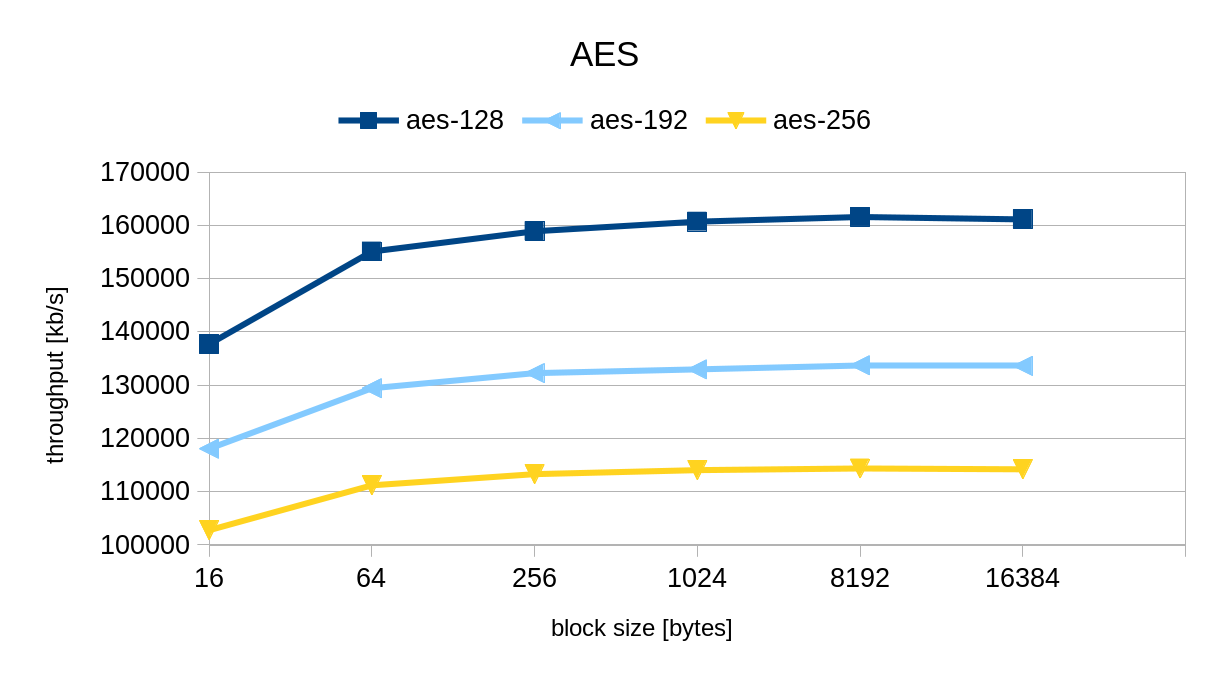
\includegraphics[width=\textwidth]{aes.png}
\end{figure}

On figure \ref{fig:aes} you can see that the larger the keys sizes the slower it gets. Whereas the throughout gets higher the larger the block size is.

\begin{figure}[htp]
    \centering
    \caption{RSA}
    \label{fig:rsa}
    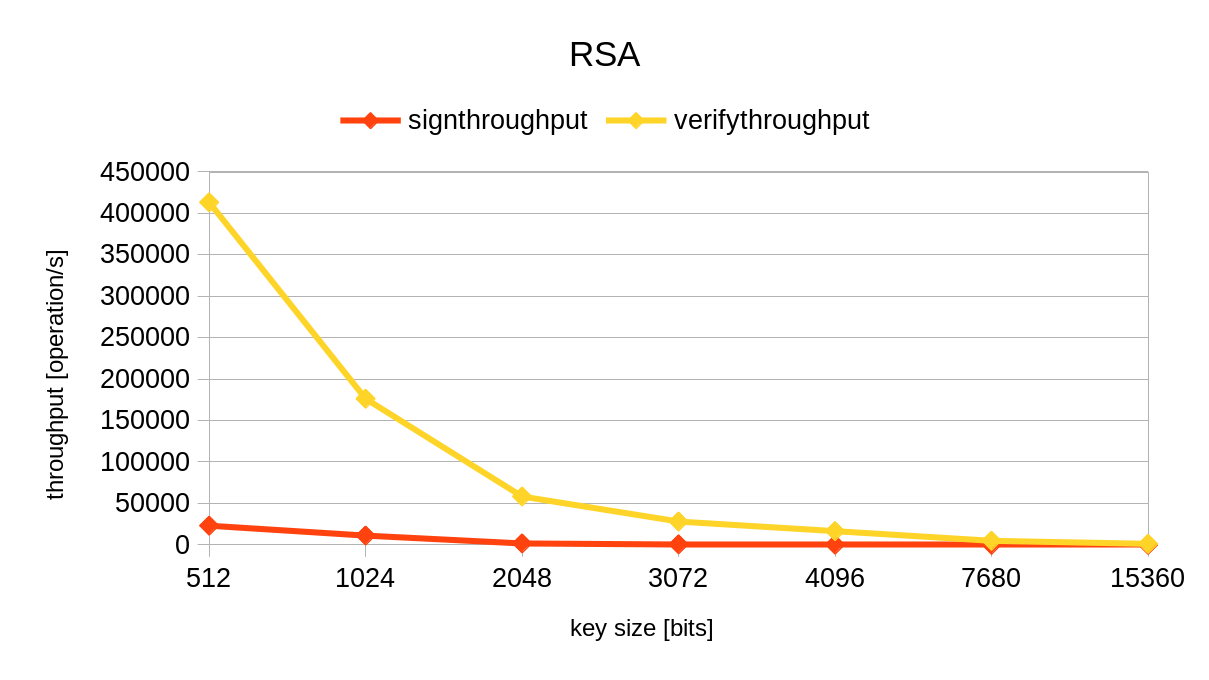
\includegraphics[width=\textwidth]{rsa.png}
\end{figure}
On figure \ref{fig:rsa} you can see that throughput is decreasing the larger the key size gets. Additionally the verification operation is significantly faster than signing.\\
Though it's hard to compare them in detail, because the speed for RSA is measured in operations whereas the speed for AES is measured in kbit/s so its two different methods. Furthermore block size and key size is also not the same. Conspicuous is that at AES the throughput is increasing with the larger block size and at RSA it's decreasing.

%\appendix
%\chapter{Appendix}
%\input{08Anhang.tex}

%%HIER ENDET DIE ARBEIT! DER REST IST KOMMENTAR MIT EIN PAAR PRAKTISCHEN FORMATIERUNGEN!!
\end{document}



%%%%%EINIGE SEHR PRAKTISCHE FORMATIERUNGSBEFEHLE UM ALLES SCHÖN UND EINHEITLICH AUSSEHEN ZU LASSEN!!%%%%%%%
%%%%%%%%%%%%%%%%%%%%%%%%%%%%%%%%%%%%%%%%%%%%%%%%%%%%%%%%%%%%%%%%%%%%%%%%%%%%%%%%%%%%%%%%%%%%%%%%%%%%%%%%%%%
%%%%%%%%%%%%%%%%%%%%%COMMENT%%%%%%%%%%%%%%%%%%%%%%COMMENT%%%%%%%%%%%%%%%%%%%%%%COMMENT%%%%%%%%%%%%%%%%%%%%%
%%%%%%%%%%%%%%%%%%%%%%%%%%%%%%%%%%%%%%%%%%%%%%%%%%%%%%%%%%%%%%%%%%%%%%%%%%%%%%%%%%%%%%%%%%%%%%%%%%%%%%%%%%%
\begin{comment}

% FORMELN UND PARAMETERBESCHREIBUNGEN
\begin{align}
\Delta \varphi = 360^\circ \cdot \frac{\Delta t}{T} = 360^\circ \cdot \Delta t \cdot f
\end{align}
wobei:
\begin{conditions} % *sternchen für zeilenübergreifende beschreibungstexte!!!
\Delta \varphi	& Phasenverschiebung \\
\Delta t		& Zeitdifferenz zwischen Eingangsspannung und gedämpfter Ausgangsspannung\\
T				& Periodendauer der Eingangsspannung \\
f				& Frequenz der Eingangsspannung
\end{conditions}

% Aufrechte griechische Buchstaben für Einheiten
\upmu
\upalpha
...etc

% BILDER EINFÜGEN
\begin{figure}[h] %t=top b=bottom h=here p =eigene page
\centering
\includegraphics[width=15cm]{media/hohlleiter}
\caption{Versuchsaufbau Hohlleiter}
\label{fig:label}
\end{figure}

% MEHRERE BILDER NEBENEINANDER
\begin{figure}[h] %t=top b=bottom h=here p =eigene page 
\flushright
\subfloat[Dispersionsrelation]{\includegraphics[width=7cm]{media/dispers}}
\subfloat[Phasen- und Gruppengeschwindigkeit]{\includegraphics[width=7cm]{media/phasgrupp}}
\end{figure}

%BILDER VOM TEXT UMFLOSSEN
\begin{wrapfigure}[10]{r}{8cm}
\centering
\includegraphics[width=7cm]{media/bragg}
\caption{\textsl{Aufbau eines Bragg-Spektrometers}}
\label{fig:bragg}
\end{wrapfigure}

%TABELLEN
\begin{table}[h]
\centering
\begin{tabular}{|c|c|}
\hline
$z$ [mm] & $\Delta z$ [mm]\\
\hline
3,3 & 0 \\
4,9 & 1,6 \\
6,5 & 1,6 \\
8,0 & 1,5 \\
\hline
\end{tabular}
\caption{Position der Minima zueinander und jeweiliger gemessener Abstand}
\label{tab:label}
\end{table}

% VERBUNDENE ZELLEN IN TABELLEN
\begin{table}[h]
\centering
\begin{tabular}{|c|c|c|c|p{1cm}p{1cm}p{1cm}p{1cm}p{1cm}p{1cm}p{1cm}|}
\hline
A & B & C & D & \multicolumn{7}{|c|}{F}  \\ \hline
\multirow{ 2}{*}{1} & 0 & 6 & 230 & 35 & 40 & 55 & 25 & 40 & 35 & \\
& 1 & 5 & 195 & 25 & 50 & 35 & 40 & 45 &  &  \\ \hline
\end{tabular}
\caption{A test caption}
\label{tab:table2}
\end{table}

% MEHRERE TABELLEN NEBENEINANDER
\begin{table}[h]
\centering

\subfloat[PVC, $d=15,0\,$mm]{
\begin{tabular}[b]{|c|c|c|}
\hline
mit Platte & ohne Platte & $\Delta s$\\
\hline
3,6 & 4,85 & 1,25\\
3,55 & 4,8 & 1,25\\
3,5 & 4,75 & 1,25\\
3,55 & 4,85 & 1,3\\
\hline
\end{tabular}
}

\subfloat[PE, $d=12,2\,$mm]{
\begin{tabular}[b]{|c|c|c|}
\hline
mit Platte & ohne Platte & $\Delta s$\\
\hline
3,5 & 4,2 & 0,7\\
3,5 & 4,25 & 0,75\\
3,5 & 4,2 & 0,7\\
\hline
\end{tabular}
}

\caption{Materialproben und zugehörige Messwerte in [cm]}
\end{table}

% FLOATS ERZWINGEN = TABELLEN UND BILDER ZWINGEND EINFÜGEN
\FloatBarrier

% ABSÄTZE MIT EINSTELLBARER UND NACHTRÄGLICH GLOBAL ÄNDERBARER DISTANZ
\mypar

% PDFs ANHÄNGEN
\includepdf[pages=-]{media/protokoll}

%BILDER UND TABELLEN REFERENZIEREN
\ref{labelname}
\pageref{labelname}

%REFERENZIERUNGSREGELN ZUR ÜBERSICHTLICHKEIT
bilder: fig:label
tabellen: tab:label
gleichungen: eq:label

\end{comment}
%%%%%%%%%%%%%%%%%%%%%%%%%%%%%%%%%%%%%%%%%%%%%%%%%%%%%%%%%%%%%%%%%%%%%%%%%%%%%%%%%%%%%%%%%%%%%%%%%%%%%%%%%%%
%%%%%%%%%%%%%%%%%%%%%COMMENT%%%%%%%%%%%%%%%%%%%%%%COMMENT%%%%%%%%%%%%%%%%%%%%%%COMMENT%%%%%%%%%%%%%%%%%%%%%
%%%%%%%%%%%%%%%%%%%%%%%%%%%%%%%%%%%%%%%%%%%%%%%%%%%%%%%%%%%%%%%%%%%%%%%%%%%%%%%%%%%%%%%%%%%%%%%%%%%%%%%%%%%
